\documentclass[12pt,reqno, twoside]{amsbook}
%%%%%%%%%%%%%%%%%%%%%%%%%%%%%%%%%%%%%%%%%%%%%%%%%%%%%%%%%%%%%%%%%%%%%%%%%%%%%%%%%%%%%%%%%%%%%%%%%%%%%%%%%%%%%%%%%%%%%%%%%%%%%%%%%%%%%%%%%%%%%%%%%%%%%%%%%%%%%%%%%%%%%%%%%%%%%%%%%%%%%%%%%%%%%%%%%%%%%%%%%%%%%%%%%%%%%%%%%%%%%%%%%%%%%%%%%%%%%%%%%%%%%%%%%%%%
\usepackage{eurosym}
\usepackage{amsmath}
\usepackage{amssymb}
\usepackage{amsfonts}
\usepackage{chngcntr}
\usepackage{graphicx}
\usepackage{csquotes}
\usepackage{subcaption}
\usepackage{minted}
\usepackage[a4paper, margin=2.5cm]{geometry}
\usepackage[english]{babel}
\usepackage{fancyhdr}
\usepackage{titlesec}
\usepackage{enumitem}
\usepackage{etoolbox}
\usepackage{booktabs}
\usepackage{lscape}
\usepackage{tabularx}
\usepackage{rotating}    % for sidewaystable
\usepackage{adjustbox}   % to scale table content
\usepackage{afterpage}

\usepackage[labelfont=normalfont,textfont=normalfont]{caption}
\usepackage[table]{xcolor}
\usepackage[acronym]{glossaries}
\makeglossaries
\usepackage[style=apa,backend=biber]{biblatex}

\usepackage{svg}
\usepackage[hidelinks]{hyperref}
\hypersetup{
    linktoc=all,     %set to all if you want both sections and subsections linked
}
\usepackage{times}
\usepackage[onehalfspacing]{setspace}
\setlength{\parindent}{0.7cm}
\setlength{\parskip}{0pt}
\titlespacing{\section}{0pt}{1.5\baselineskip}{\baselineskip} % (left, before, after)
\titlespacing{\subsection}{0pt}{\baselineskip}{\baselineskip}
\titlespacing{\subsubsection}{0pt}{\baselineskip}{\baselineskip}
\fancyfoot[LE,RO]{\thepage} % Esquerda nas pares, direita nas ímpares
\setlength{\footskip}{1.25cm} % Distância ao fundo da página



% you may need to uncomment the command below if you use eps format for figures
%\usepackage{epstopdf}


\makeatletter
    \def\section{\@startsection{section}{1}%
      \z@{.5\linespacing\@plus.7\linespacing}{.25\linespacing}%
      {\normalfont\bfseries\flushleft}}
    \def\subsection{\@startsection{subsection}{2}%
      \z@{.5\linespacing\@plus.7\linespacing}{.25\linespacing}%
      {\normalfont\bfseries\flushleft}}
    \def\subsubsection{\@startsection{subsubsection}{3}%
      \z@{.5\linespacing\@plus.7\linespacing}{.25\linespacing}%
      {\normalfont\bfseries\flushleft}}

\makeatother
\setcounter{MaxMatrixCols}{10}

\providecommand{\U}[1]{\protect\rule{.1in}{.1in}}
\theoremstyle{plain}
\newtheorem{acknowledgement}{Acknowledgement}
\newtheorem{algorithm}{Algorithm}[chapter]
\newtheorem{axiom}{Axiom}[chapter]
\newtheorem{case}{Case}[chapter]
\newtheorem{claim}{Claim}[chapter]
\newtheorem{conclusion}{Conclusion}[chapter]
\newtheorem{condition}{Condition}[chapter]
\newtheorem{conjecture}{Conjecture}[chapter]
\newtheorem{corollary}{Corollary}[chapter]
\newtheorem{criterion}{Criterion}[chapter]
\newtheorem{definition}{Definition}[chapter]
\newtheorem{example}{Example}[chapter]
\newtheorem{exercise}{Exercise}[chapter]
\newtheorem{lemma}{Lemma}[chapter]
\newtheorem{notation}{Notation}[chapter]
\newtheorem{problem}{Problem}[chapter]
\newtheorem{proposition}{Proposition}[chapter]
\newtheorem{remark}{Remark}[chapter]
\newtheorem{solution}{Solution}[chapter]
\newtheorem{summary}{Summary}[chapter]
\newtheorem{theorem}{Theorem}[chapter]
\numberwithin{equation}{chapter}

\newcommand{\tabref}[1]{\textbf{Table~\ref{#1}}} 
\newcommand{\figref}[1]{\textbf{Figure~\ref{#1}}}
\counterwithout{figure}{chapter}
\counterwithout{table}{chapter}
\renewcommand{\thefigure}{\arabic{figure}}

\numberwithin{section}{chapter}
\fancyhead{}
\fancyfoot{}
\pagestyle{fancy}
\fancyfoot[LE,RO]{\thepage}

\makeatletter
\def\ps@plain{\ps@empty
 \def\@evenfoot{%
   \normalfont\scriptsize
   \rlap{\thepage}\hfil
   }%
 \def\@oddfoot{%
   \normalfont\scriptsize \hfil
   \llap{\thepage}}%
}
\makeatother
\renewcommand{\headrulewidth}{0pt}
\renewcommand{\footrulewidth}{0pt}

\newglossarystyle{glostable}
{%
    \renewenvironment{theglossary}
    {
        \begin{longtable}{|p{0.25\textwidth}|p{0.025\textwidth}|p{0.7\textwidth}|}
    }
    { \end{longtable} }

    \renewcommand*{\glossaryheader}
    {
        \hline
        \textbf{Symbol} & - & \textbf{Description} \\
        \hline
    }

    \renewcommand*{\glsgroupheading}[1]{}
    \renewcommand*{\glsgroupskip}{}
    \renewcommand{\glossentry}[2]
    {
        \glossentryname{##1} & - & \glossentrydesc{##1} \\
        \hline

    }
    \renewcommand*{\subglossentry}[3]{}
}
\begin{document}
\begin{titlepage}
    \raggedright
    \includegraphics[width=0.4\textwidth]{assets/logo_iscte_ista.png} \\[1cm]
    
    \Large
    \textbf{\LARGE GitDash - Software Architecture and Design - Project Report} \\[0.5cm]

    Master's in Computer Science and Business Management \\[2cm]
    
    Gonçalo Gonçalves Miranda \\[0.5cm]
    
    
    \raggedright
    Teacher:\newline
    PhD José Pereira dos Reis\newline
    Assistant Professor, ISCTE-IUL \newline

    \vfill
    \centering
    \large
    ISCTE – Instituto Universitário de Lisboa \\
    \centering
    January, 2026
\end{titlepage}


\frontmatter
\addtocontents{toc}{\setcounter{tocdepth}{3}    % include subsubsections in the ToC
\setcounter{secnumdepth}{3} % (optional) number subsubsections as well
}

\tableofcontents

\listoffigures
\listoftables

\printglossary[type=\acronymtype,style=glostable,title={List of Acronyms}]

\mainmatter

\hyphenation{wri-te he-re pro-per hy-phe-ni-za-tion
}%

\setcounter{page}{1} \pagenumbering{arabic}

\chapter{Introduction}
\noindent In modern days software development, GitHub plays a central role in coordinating distributed teams and managing complex 
projects, as the development process is increasingly collaborative and data-driven. While it provides a wide range of 
analytics and repository insights out of the box, Github often displays them across multiple views and not by highlighting 
individual contributor activity in a unified, centralized way. As projects grow in size and complexity,it can be benefitial 
to clearly view into participation patterns, contribution levels, and recent activity.

This project, that was developed for the Software Architecture and Design course at ISCTE-IUL, targets precisely that need by 
proposing and implementing an API-based user dashboard for GitHub projects, focused on aggregating and visualizing contributor-level 
metrics in an intuitive, responsive interface. By integrating directly with the GitHub API and using the platform's OAuth, the 
system is able to securely access repository data and automatically identify all contributors involved in a given project. For each 
contributor, the application generates a personalized dashboard that presents key indicators about the contributors envolvment in 
the repository's code development.

The solution emphasizes not only data collection, but also meaningful presentation, as there was also a focuse to graphically 
present the gathered data in comprehensible ways, providing better insights to the contributors about their performance. This was 
achieved by using both line charts and pie charts.

\chapter{Project Development}
\noindent This section describes how the system was developed, focusing on how the proposed architecture and implementation choices 
address the project's functional requirements, as well as how it fulfills common quality attributes. The solution was developed as a 
full-stack web application composed of a frontend client written in Next.js and a backend API, designed with NestJS in order to 
collect, process, and visualize data from GitHub at both repository and contributor levels. This chapter also details design 
decisions and some trade-offs made during the development process, in order to achieve a system that fulfills the initially defined functional requirements.

\section{Functional Requirements}
\noindent This section goes into how the functional requirements defined for the project were fullfilled by the developed system. 
All the requirements were implemented by coordinating the client-side application (the frontend) and the server-side API 
(the backend), where the former is responsible for user interaction and visualization, and the latter manages authentication, 
data retrieval, aggregation, and integration with the GitHub API.

\subsection{Authentication via GitHub OAuth}
\noindent The system supports user authentication through GitHub OAuth 2.0, allowing users to use their GitHub accounts to sign.
The authentication flow starts on the frontend, with a user click on the login button, which then initiates a redirection to GitHub’s 
authorization service that, upon successful authentication, redirects the user to one of the backend routes, where an application 
session is generated and passed on to the frontend as a cookie, that is later used to authenticate subsequent requests. Route 
protection is implemented on the frontend's middleware layer, at the context layer and on the backend's controller layer, which 
guarantees that any unauthenticated user is unable to access protected content, and session validity is continuously enforced to 
prevent unauthorized access and force the users to re-authenticate themselves as soon as possible. It is also possible for a user 
to terminate their session through a logout mechanism, ensuring proper session lifecycle management.

\subsection{Selection of a Specific Repository}
\noindent After authentication, users can select a Github repository from a list of their own repositories, or search public repositories 
either by entering their URL or name. Once a repository is selected, the frontend maintains the selection consistently across views 
and uses it as the context for subsequent data retrieval. This mechanism enables seamless navigation between repositories and ensures
 that all displayed data remain synchronized with the currently selected project.

\subsection{Automatic Identification of Project Contributors}
\noindent After the repository selection, all its contributors are dynamically fetched and associated with the project. Contributor 
data is presented incrementally to support repositories with a large number of contributors. The system maintains an updated list of 
contributors and uses this data for further exploration and metric generation.

\subsection{Individual Contributor Dashboard with Metrics}
\noindent After display all contributors on a specific repository, the system allows the user to select a contributor to explore. 
When the selection happens, an individual dashboard that presents contributor metrics relevant to project activity and 
participation is fetched from the backend (which then fetches data from GitHub's APi and processes it into structured, insightful
responses), utilizing parallelized API calls in order to smoothen the data loading. These metrics 
include the number of commits, lines of code added and removed, issues opened and closed, pull requests submitted and approved,
recent development activity by week, and PR conversion rate.

\subsection{Graphical Visualizations}
\noindent Graphical visualizations is supported by the system, enabling intuitive exploration of contribution data, via the utilization 
of line charts and pie charts. This enables users to identify trends, distributions, and relative contributions at a glance. 
Visualizations are generated from aggregated data and are dynamically updated according to repository and/or contributor context 
changes.

\subsection{Responsive and Intuitive User Interface}
\noindent The user interface is designed to be responsive and intuitive, being easy and intuitive to interact with and adaptable to 
different screen sizes. Navigation, search, and dashboard interactions are designed to support efficient exploration of repository 
data. The UI elements are structured to provide clear feedback and maintain usability across devices, ensuring that contribution 
insights remain accessible to a wide a variety of users and usage scenarios.

\section{Solution Architecture}
\subsection{High-level Architecture}
The system follows a client-server architecture composed, of a web frontend application designed with Next.js 
and a backend API, with GitHub's APIs acting as the external data source. At a high level 
(as illustrated in \figref{fig:high_lvl_arch}), the frontend is responsible for authentication initiation, 
navigation, and the visualization of data, while the backend is used to process authentication logic, data 
collection, aggregation, caching, and response shaping. Redis is also used as a cache for analytics data and 
for session data.
\begin{figure}[htbp]
    \centering
    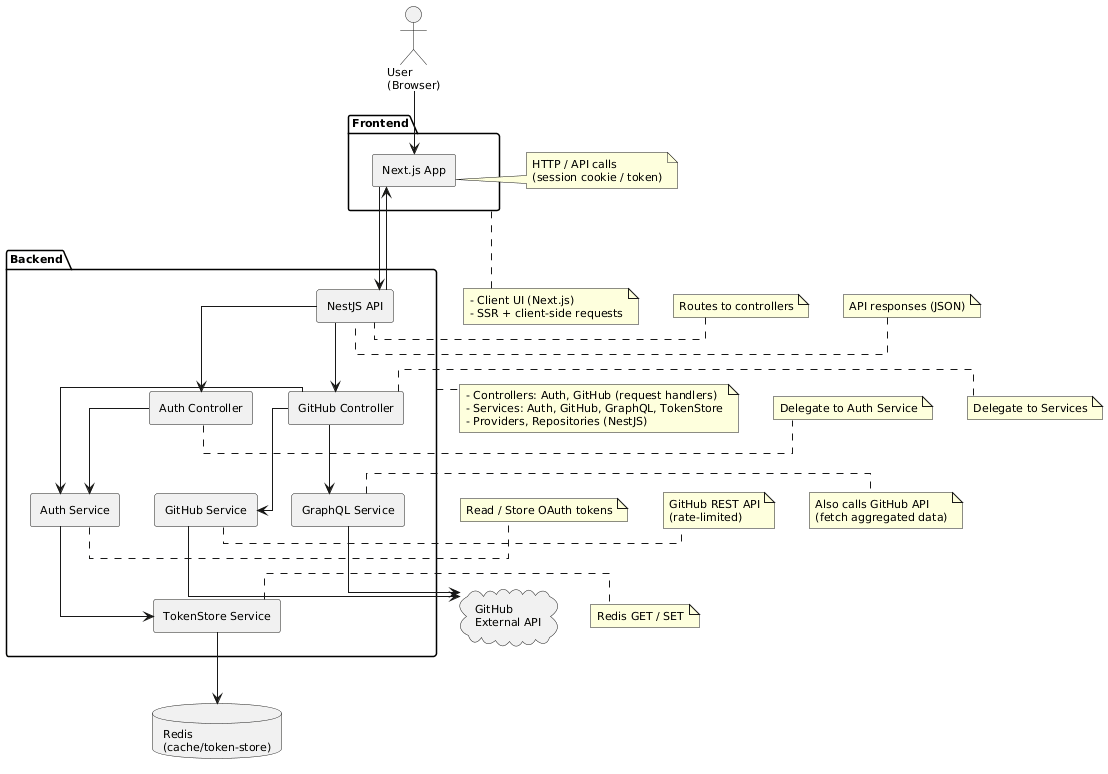
\includegraphics[width=0.7\textwidth]{assets/high-level-architecture.png}
    \caption{High Level Architecture}
    \label{fig:high_lvl_arch}
\end{figure}

\subsection{Architecture Design Patterns}
\noindent This project leverages several well-established design patterns across both the backend and the frontend components, in order to 
improve modularity, maintainability, scalability, and clarity of responsibility. Rather than just being applied individually, these 
patterns naturally emerge from the architectural choices made — particularly the use of the frameworks in use.

The backend architecture heavily benefits from NestJS’s opinionated design, which encourages the use of proven enterprise patterns, 
while The frontend design patterns applied to the frontend are the natural outcome of using Next.js (and React, its base), focusing 
on state management, UI composition, and interaction control.

\subsubsection{Dependency Injection Pattern}
\noindent The Dependency Injection pattern is applied through NestJS’s \texttt{@Injectable()} mechanism and constructor-based 
injection. Core services, including authentication, GitHub integration, GraphQL Integration, token storage, and data mapping, are 
injected into dependent components rather than being instantiated directly, which decouples components from concrete implementations, 
enhanced testability by enabling mocking or substitution of dependencies, and improves maintainability by localizing changes to 
specific services without affecting dependent modules.

\subsubsection{Singleton Pattern}
\noindent On the backend, NestJS providers are instantiated as singletons by default within the application context. As a result, all the services that are 
injected are only created once and reused throughout the application lifecycle. Due to this behaviour, shared resources, such as 
Redis connection, are consistently and efficiently managed, reducing instantiation overhead and maintaining a single, coherent 
state across requests.

This pattern is, however, also used on the frontend to control global application state, by instantiation a single React Context 
provider, which ensures consistent data access across components and aids in avoiding prop drilling.

\subsubsection{Decorator Pattern}
\noindent NestJS’s decorator-based programming model is extensively used, as built-in decorators such as @Controller, @Get, and 
@UseGuards simplify request routing and security enforcement. Additionally, a custom decorators can be created and, in this case, 
one is used to extract session identifiers from JWT payloads, reducing boilerplate code inside controllers and improving readability 
and maintainability.

\subsubsection{Guard Pattern}
\noindent
The Guard pattern is applied by the backend to enforce authorization rules on protected resources, using the @UseGuard
decorator. A custom JWT-based guard intercepts incoming requests and evaluates whether or not the requesting client is authorized
 before allowing access to controller endpoints, which enables the usage of access control policies consistently across the 
 application and helps avoid duplicate checks within individual controllers.

\subsubsection{Middleware Pattern}
\noindent Middleware is used by the frontend (almost as a guard) at the application level to handle cross-cutting concerns that 
apply to all incoming requests before they are processed by any route. These concerns include request preprocessing tasks such as 
CORS configuration, cookie parsing, and session-related handling, which also aids the clear separation between infrastructural concerns and business logic, improving maintainability and readability.

\subsubsection{Facade Pattern}
\noindent Both the main services used by the backend, such as the GitHub service and authentication service act as facades, as they 
provide simplified, high-level methods that encapsulate complex logic involving multiple API calls, data transformations, 
and caching steps. Controllers can be abstracted from business logic by interacting with these services through concise method calls, 
without needing to understand the underlying complexity of GitHub APIs.

\subsubsection{Mapper Pattern}
\noindent On the backend, the dedicated mapper service transforms raw GitHub API responses into internal domain models used by the application, 
which isolates the system from changes in external API schemas and ensures the stability of the date structures the internal 
application logic interacts with, while also keeping transformation logic centralized.

\subsubsection{Repository Pattern}
\noindent The backend's token store service applies a Repository-like pattern by abstracting persistence operations related to 
sessions, OAuth state, and cached repository statistics by exposing domain-specific methods for creating, retrieving, and deleting 
stored data, being the only point of direct interaction with the underlying storage mechanism (in this case, Redis) within the whole 
application. This abstraction improves maintainability and allows the persistence layer to be modified or replaced without impacting 
higher-level services.

\subsubsection{Caching Pattern}
\noindent Caching is implemented on the backend using Redis with configurable time-to-live (TTL) values to temporarily store session data and 
computed GitHub statistics (which, for bigger repositories, is a call that can last for a few seconds, which isn't ideal). This 
follows the Caching pattern by reducing redundant external API calls and improving response times. Cached entries are automatically 
expired by Redis, which ensures data freshness while maintaining efficient resource usage.

\subsubsection{Factory Pattern}
\noindent The Redis client on the backend is instantiated using a factory function that centralizes configuration concerns such as connection 
options, retry strategies, and event registration, which allows the application to ensure consistent Redis client setup and 
simplifies future modifications to the persistence configuration without affecting dependant services.

\subsubsection{Observer Pattern}
\noindent The application's frontend implements the observer pattern in multiple forms, ranging from a custom hook that periodically 
observes session validity and updates global state accordingly, which allows the UI to react to authentication changes, to the usage 
of the IntersectionObserver API in order to monitor scrolling behavior on the contributors navbar and trigger incremental loading of 
contributors, enabling efficient infinite scrolling.

\subsubsection{Composite Pattern}
\noindent The individual UI components on the application's frontend are composed hierarchically into higher-level structures such as 
dashboards, summary panels, and navigation layouts and, ultimately, into pages. This composition enables complex interfaces to be 
designed from simpler building blocks, allowing consistent behavior across pages while maintaining flexibility in the generation of 
new pages.

\subsubsection{Command and Cancellation Pattern}
\noindent Network requests executed by the frontend are treated as cancellable commands through the use of abort controllers, as
this allows in-flight requests to be explicitly cancelled when they become obsolete, such as during rapid search input changes. By 
controlling a request's lifecycle, processing stale responses can be avoided and improves both performance and data correctness.

\subsubsection{Debounce Pattern}
\noindent The application's frontend uses debounce mechanisms in user interactions, such as window resize events and search input 
handling. By delaying execution until user activity stabilizes, the application reduces unnecessary re-renders and network requests, 
leading to a better user experience and to improvals on resource usage efficiency.

\subsubsection{Template Pattern}
\noindent Reusable UI Components, such as buttons, inputs, and dialog components (some from ShadCN's library), follow a 
template-style approach that defines the component's structure, behavior, and styling throughout the application in a consistent 
manner. By encapsulating common interaction patterns within these primitives, the frontend is able to enforce an uniform user 
experience and reduces boilerplate, improving maintainability and UI extensibility.

\subsection{Architecture Quality Attributes}
\noindent
In addition to the system's functional requirements, the proposed architecture was designed to support a set of key software 
quality attributes that contribute to the system’s robustness, extensibility, and long-term sustainability. These 
attributes are aligned with widely accepted quality attributes, such as security, performance, usability, maintainability, and 
deployability. The following sections explain which attributes are supported by the current architecture and how they were implemented.

\subsubsection{Security and Authentication}

Security is a critical quality attribute for most systems, especially if third-party platforms are integrated or if user identity 
data is handled. The application implements secure authentication and session management across both the frontend and the backend.

On the frontend, authentication is handled through the GitHub OAuth flow. The login component redirects users to a configured 
authentication endpoint (on Next.js' server side routes, where it then re-directs the user to Github's OAuth flow, which finally 
redirects the users to a route on the backend which redirects to the main dashboard route on the frontend), while a middleware 
enforces server-side route protection, that validates sessions against the backend API. Session cookies are handled consistently 
being included in all requests made credential-inclusive, and logout operations explicitly trigger the backend route to invalidate 
the server-side session. Client-side session monitoring is implemented through a dedicated session watcher hook, which periodically 
validates session state and proactively handles session expiration.

On the backend, OAuth 2.0 is used to delegate authentication to GitHub, eliminating the need to store user credentials locally. 
Sessions are managed using signed JWTs with configurable expiration times, stored and validated through Redis, while secure cookie 
settings (HTTP-only, SameSite policies, and TLS support) mitigate common web vulnerabilities, such as XSS and CSRF.

The combination of the mechanisms implemented between the frontend and the backend promotes strong security for the system.

\subsubsection{Performance and Scalability}

When dealing with repositories that may have a large ammount of contributors and, therefore, a huge quantity of data associated with 
them, performance and scalability are essential quality attributes, as the system must be able to proccess these use-cases as well as 
small repositories.

On the frontend, responsiveness is achieved through a combination of debounced UI hooks, responsive, external layout components, 
and efficient rendering strategies. Charts are rendered using responsive containers, and layout adjustments rely on debounced window 
size detection to avoid unnecessary reflows. Data fetching is optimized through parallel requests using typescript's \texttt{Promise.All}, 
in-flight request cancellation via AbortController, and debounced search inputs, while the contributor list supports infinite 
scrolling with pagination through the use of the IntersectionObserver API, enabling efficient handling of large datasets.

On the backend, the usage of Redis as a cache to store session data and computed repository statistics 
are cached with configurable TTLs, results in a smaller number of repeated calls to the GitHub API (which also helps the system avoid 
getting the rate-limited by Github). Pagination is implemented for API responses such as contributor lists, allowing the system to 
scale to repositories with large contributor bases, while still supporting smaller repositories. Besides this, GitHub's GraphQL API 
was also used so that only required data fields were fetched, reducing payload sizes and improving response times substantially. 
Besides this, parallel computing was also used in order to perform concurrent API requests, which significantly reduces latency when 
multiple resources are required.

Due to these decisions, the system is responsive under increased load and scales effectively with repository size.

\subsubsection{Reliability and Availability}

A system's reliability is defined as the its ability to correctly and continuosly operate, regardless of the existence of partial 
failures. This is the one of the core characteristics that was taken into consideration when developing this specific system. 
Redis connections are configured with keep-alive mechanisms, health checks, and retry strategies using exponential backoff, helping 
to maintain session availability during transient network issues while API interactions with GitHub are wrapped in structured error 
handling logic, allowing partial data to be returned even when some requests fail, rather than causing complete request failures.
Besides this, session expiration and validation mechanisms are also implemented, in order to make the system more reliable, by 
ensuring that stale or invalid sessions are detected and gracefully handled. Basic logging of infrastructure events, such as Redis 
connection state changes, provides operational visibility and facilitates the diagnosing of runtime issues.

\subsubsection{Usability and Accessibility}
As for the system's accessibility, certain ShadCN components were used in for the UI, which provide out of the box 
accessibility support, such as focus-visible styling and basic ARIA attributes, such as aria-invalid handling in form elements. 
Alongside this, images on the custom components include alternative text to support assistive technologies.
Regarding the usability, a user-friendly UI was developed using both ShadCN and custom components, as well as debounced input 
handling for smoother interactions was implemented. Even though usability was something that was focused and achieved on this system, 
accessibility is only partially achieved, as not all the components utilized support assistive technologies.

\subsubsection{Maintainability and Extensibility}

Systems that are envisioned to evolve over time must be maintainable and extensible. To achieve these characteristics, both the 
frontend and the backend codebases are written entirely with TypeScript as the code-base's main language, providing strong type 
safety and reducing runtime errors. The frontend was was built to be modular and component-based and the 
principal of the separation of concerns was followed, including reusable UI primitives, chart components, and a typed global state 
managed through React context. This structure, alongside the usage of Next.js, which improves maintainability and extensibility 
through its opinionated project structure and built-in routing and rendering conventions, reduces architectural complexity and 
allows new pages, components, metrics, charts, or dashboard sections to be added with minimal impact on existing code, further 
improving the maintainability and extensibility of the system.

As for the backend, it adopts a service-oriented architecture built on NestJS, a framework that leverages dependency injection to
 promote loose coupling and testability. The main features are separated into dedicated services, improving readability and 
 facilitating extensions. Besides this, configuration is fully externalized through environment variables, enabling changes across 
 environments without code modifications.

\subsubsection{Error Handling and Observability}

As for the error handling and observability, the frontend includes basic validation of responses and error propagation for network 
requests with fallback behaviors in place to prevent UI crashes. However, there is no integrated monitoring, structured logging, or 
external error-reporting service.

On the backend, API calls are protected with try-catch blocks and defensive logic to prevent cascading failures. Events on the 
infraestructure level, such as the ones related to Redis connectivity, are logged to provide insight into system health. 

While this approach is sufficient for a small project, observability could be improved through structured logging and centralized 
monitoring in a production setting.

\subsubsection{Data Handling and Privacy}

The system also looked to preserve data privacy by minimizing the storage and exposure of personal data. The frontend stores user and 
session data in memory through the global context and does not persist it locally beyond the cookies required for authentication, 
which are also used for session management. The content of this cookie is a JWT token, which only contains a session and user id,
the authenticated user's username and the token issue and expiration date. Besides that, session-sensitive requests explicitly 
disable caching and consistently include credentials to ensure correctness and privacy.

As for the backend, sensitive data such as access tokens and session information are stored securely in Redis and are automaticaly
 expirated, according to the TTL set to each entry. No unnecessary data is persisted beyond what is required for authentication, 
 aligning with data minimization principles.

\subsubsection{Deployability and Portability}
\noindent Reliable builds and deployments across environments are ensured by deployability and portability.

As Next.js is the framework used for the frontend, which supports environment-driven configuration, it is 
compatible with standard CI/CD pipelines and modern hosting platforms.

As for the backend, it was built on NestJS, which is a production-ready Node.js framework designed for 
scalable server-side applications. Dependency management is handled via pnpm with lock files, ensuring 
reproducible builds across environments. Environment-based configuration is also supported, which eases
deployments.

\subsubsection{Testing and Quality Assurance}

Testing is an important quality attribute related to reliability and maintainability. The backend includes a configured Jest testing
 infrastructure with support for unit and end-to-end tests. The frontend can also easily utilize an external library for such 
 purpose. However, neither the frontend nor the backend implement unit, integration or end-to-end tests.

While testing is not comprehensively implemented, the existing architecture supports the introduction of automated testing 
frameworks without major refactoring, representing a clear path for future quality improvements.

\subsection{Solution Trade-offs}
\noindent Several trade-offs were made during development to balance accuracy, performance, and implementation 
complexity, being the most notable example the calculation of repository member counts. As GitHub 
distinguishes between organization members, collaborators, and contributors, and not all contributors 
necessarily have associated GitHub user accounts. To ensure the data regarding member count and actual members 
is consistent, anonymous contributors are not taken into consideration when counting the members. This 
simplification leads to a difference in contributor count between Gitdash's member count and Github's, as 
the latter also takes into consideration anonymous users, which can't be fetched via API in order to get the 
statistics. Taking these users into consideration would break the app, as they have no statistics associated in Github's API.
This trade-off was considered acceptable given the project's primary focus on comparative contribution 
patterns rather than exhaustive contributor enumeration, while ensuring predictable behavior across both 
small and big repositories.

\chapter{Conclusion}
\noindent This project successfully delivered a full-stack system for analyzing and visualizing GitHub 
repository and contributor activity. By combining a modular frontend architecture with a scalable backend service
 layer, the solution provides an effective platform for exploring activity in a structured and user-friendly 
 manner.

From a technical standpoint, the project successfully integrates modern web technologies with third-party APIs, 
highlighting challenges related to data aggregation, pagination, and rate-limiting. The architectural decisions 
adopted throughout the project support several quality attributes, adding up to the system's quality.

Overall, the system meets its defined objectives and provides a solid foundation for any possible future work 
in repository analytics and developer productivity assessment. It also reinforces the importance of clear 
architectural separation and informed trade-offs when designing data-intensive web applications.


Overall, the system meets its defined objectives and provides a solid foundation for any possible future work 
in repository analytics and developer productivity assessment. It also reinforces the importance of clear 
architectural separation and informed trade-offs when designing data-intensive web applications.

\appendix

\chapter{User Stories}
\section{GitHub OAuth Login (Frontend)}
\begin{itemize}
  \item Description: As a user, I want to initiate login using GitHub so that I can authenticate into the dashboard.
  \item Story Point Estimate: 3 
  \item Acceptance Criteria: 
    \begin{itemize}
      \item Login button redirects to GitHub OAuth.
      \item Handles redirect callback.
      \item Redirects to \texttt{/dashboard} on success.
    \end{itemize}
\end{itemize}

\section{GitHub OAuth login (Backend)}
\begin{itemize}
  \item Description: As a system, I want to handle GitHub OAuth authentication so that secure sessions can be created.
  \item Story Point Estimate: 5
  \item Acceptance Criteria: 
    \begin{itemize}
      \item OAuth code exchanged for access token
      \item User identity resolved from GitHub
      \item Secure session cookie created
      \item Invalid flows are rejected
    \end{itemize}
\end{itemize}

\section{Session-protected routing (Frontend)}
\begin{itemize}
  \item Description: As a user, I want protected routes to require authentication so that unauthorized access is blocked.
  \item Story Point Estimate: 5
  \item Acceptance Criteria: 
    \begin{itemize}
      \item Middleware blocks protected routes
      \item Invalid session displays session dialog, in order to redirect to /login
      \item Valid sessions allow navigation
    \end{itemize}
\end{itemize}

\section{Session validation endpoint (Backend)}
\begin{itemize}
  \item Description: As a system, I want to validate active sessions so that frontend can enforce access control.
  \item Story Point Estimate: 2
  \item Acceptance Criteria: 
    \begin{itemize}
      \item /session endpoint validates cookie
      \item Returns valid/invalid status, username and TTL
      \item Handles expired sessions correctly
    \end{itemize}
\end{itemize}

\section{Logout (Frontend)}
\begin{itemize}
  \item Description: As a user, I want to log out so that my session is terminated.
  \item Story Point Estimate: 1
  \item Acceptance Criteria: 
    \begin{itemize}
      \item Logout clears client state
      \item User redirected to landing page
    \end{itemize}
\end{itemize}

\section{Logout (Backend)}
\begin{itemize}
  \item Description: As a system, I want to invalidate sessions so that logged-out users cannot reuse them.
  \item Story Point Estimate: 1
  \item Acceptance Criteria: 
    \begin{itemize}
      \item Session cookie invalidated/Removed
      \item Server-side session cleared
    \end{itemize}
\end{itemize}

\section{Search repositories (Frontend)}
\begin{itemize}
  \item Description: As a user, I want to search repositories so that I can select one to analyze.
  \item Story Point Estimate: 3
  \item Acceptance Criteria: 
    \begin{itemize}
      \item Search input should be smooth (debounce)
      \item Loading skeletons shown
      \item Results update without stale data
    \end{itemize}
\end{itemize}

\section{Search repositories (Backend)}

\section{Select repository (Frontend)}
\begin{itemize}
  \item Description: As a user, I want to select a repository so that I can view its dashboard.
  \item Story Point Estimate: 2
  \item Acceptance Criteria: 
    \begin{itemize}
      \item Clicking repo navigates to /dashboard/{owner}/{repo}
      \item Selected repo stored in global state
      \item Displays basic repository info
    \end{itemize}
\end{itemize}

\section{Repository metadata fetch (Backend)}
\begin{itemize}
  \item Description: As a system, I want to fetch repository metadata so that dashboards have context.
  \item Story Point Estimate: 3
  \item Acceptance Criteria: 
    \begin{itemize}
      \item Fetch repository metadata by owner/name
      \item Return consistent schema
      \item Handle edge cases
    \end{itemize}
\end{itemize}

\section{Repository overview dashboard (Frontend)}
\begin{itemize}
  \item Description: As a user, I want to see repository statistics so that I can understand activity at a glance.
  \item Story Point Estimate: 5
  \item Acceptance Criteria: 
    \begin{itemize}
      \item Commits, issues, PRs shown
      \item Error states handled
      \item Responsive layout
    \end{itemize}
\end{itemize}

\section{Repository analytics aggregation (Backend)}
\begin{itemize}
  \item Description: As a system, I want to aggregate repository analytics so that the dashboard has unified data.
  \item Story Point Estimate: 8
  \item Acceptance Criteria: 
    \begin{itemize}
      \item Aggregate commits, issues, PRs
      \item Return data in a consistent schema
    \end{itemize}
\end{itemize}

\section{Activity over time chart (Frontend)}
\begin{itemize}
  \item Description: As a user, I want to view activity trends over time so that I can analyze evolution.
  \item Story Point Estimate: 3
  \item Acceptance Criteria: 
    \begin{itemize}
      \item Line chart renders weekly data
      \item Tooltip shows detailed metrics
      \item Responsive resizing
    \end{itemize}
\end{itemize}

\section{Activity timeline endpoint (Backend)}
\begin{itemize}
  \item Description: As a system, I want to provide time-series activity data so that charts can be rendered.
  \item Story Point Estimate: 5
  \item Acceptance Criteria: 
    \begin{itemize}
      \item Weekly aggregation supported
      \item Uses caching where possible
    \end{itemize}
\end{itemize}

\section{PR conversion pie chart (Frontend)}
\begin{itemize}
  \item Description: As a user, I want to see PR conversion rates so that I understand contribution outcomes.
  \item Story Point Estimate: 2
  \item Acceptance Criteria: 
    \begin{itemize}
      \item Pie chart shows merged/closed/open
      \item Supports counts and percentages
      \item Comprehensive UI
    \end{itemize}
\end{itemize}

\section{PR conversion metrics (Backend)}
\begin{itemize}
  \item Description: As a system, I want to calculate PR conversion metrics so that contribution efficiency is visible and comprehensible by the frontend.
  \item Story Point Estimate: 3
  \item Acceptance Criteria: 
    \begin{itemize}
      \item Count merged, closed, open PRs
      \item Filtered by contributor
    \end{itemize}
\end{itemize}

\section{List contributors (Frontend)}
\begin{itemize}
  \item Description: As a user, I want to see repository contributors so that I can analyze participation.
  \item Story Point Estimate: 3
  \item Acceptance Criteria: 
    \begin{itemize}
      \item Contributors list paginated
      \item Contributor count accurate
      \item Allow pagination when there are more users than the ones displayed
      \item Filtering does not break pagination
    \end{itemize}
\end{itemize}

\section{Fetch contributors (Backend)}
\begin{itemize}
  \item Description: As a system, I want to fetch contributors from GitHub so that contributor analytics are possible.
  \item Story Point Estimate: 5
  \item Acceptance Criteria: 
    \begin{itemize}
      \item Paginated GitHub API usage
      \item Normalized contributor data
      \item Avoids Github’s rate-limit
    \end{itemize}
\end{itemize}

\section{Contributor search (Frontend)}
\begin{itemize}
  \item Description: As a user, I want to search contributors so that I can find specific users.
  \item Story Point Estimate: 2
  \item Acceptance Criteria: 
    \begin{itemize}
      \item Client-side filtering
      \item No stale UI updates
    \end{itemize}
\end{itemize}

\section{Contributor detail view (Frontend)}
\begin{itemize}
  \item Description: As a user, I want to view contributor details so that I can assess impact.
  \item Story Point Estimate: 3
  \item Acceptance Criteria: 
    \begin{itemize}
      \item Shows commits, PRs submitted and approved, lines added and removed and issues opened and closed by the user
      \item Navigable from contributors list
      \item Display loading states appropriately
    \end{itemize}
\end{itemize}

\section{Contributor analytics aggregation (Backend)}
\begin{itemize}
  \item Description: As a system, I want to aggregate contributor activity so that detailed metrics are available.
  \item Story Point Estimate: 8
  \item Acceptance Criteria: 
    \begin{itemize}
      \item Fast response times
      \item Supports contributor + repository filters
      \item Supports caching
      \item Supports retries for asynchronous endpoints from Github’s API
    \end{itemize}
\end{itemize}

\section{Redis caching layer (Backend)}
\begin{itemize}
  \item Description: As a system, I want to cache GitHub responses so that latency and rate limits are reduced.
  \item Story Point Estimate: 5
  \item Acceptance Criteria: 
    \begin{itemize}
      \item TTL-based caching implemented
      \item Should handle sessions
      \item Should handle data chaching
      \item Graceful fallback on cache miss
    \end{itemize}
\end{itemize}

\section{GitHub API error resilience (Backend)}
\begin{itemize}
  \item Description: As a system, I want to handle GitHub API edge cases so that the app remains usable..
  \item Story Point Estimate: 3
  \item Acceptance Criteria: 
    \begin{itemize}
      \item Handles 202 stats responses
      \item Uses cached data when possible
    \end{itemize}
\end{itemize}

\end{document}
